\section{Mathematical Methods}

A small number of mathematical methods which may not be familiar to the reader are used within this thesis. They are outlined below.

\subsection{K-means clustering}

\subsection{Principal Component Analysis}

\glsreset{PCA}
\gls{PCA} is a dimensionality reduction method, used to to reduce the number of variables within a dataset whilst retaining as much of the variance as possible, and often used to identify the correlated roots of variance.

It is used extensively within the study of daylight \glspl{SPD} and \glspl{SRF}. 

In eras where the transmission of large datasets was troublesome, dimensionality reduction methods such as \gls{PCA} held value as a method to summarise a dataset, with the understanding that a reader could reconstruct a pseudo-dataset with minimal data-loss from the provided principal components. One such example is the work of \citet{judd_spectral_1964} where only the mean and first four 'characteristic vectors' are provided\footnote{This is not technically \gls{PCA} but the related technique of \citet{morris_objective_1954}.}. The data from \citet{judd_spectral_1964} is replotted in Figure \ref{fig:Judd} and it can be seen that for their dataset this description does seem to offer a sensible summary of the data: the shape of the mean can be seen, and it can be seen that the main variation further than 

\begin{figure}[htbp]
 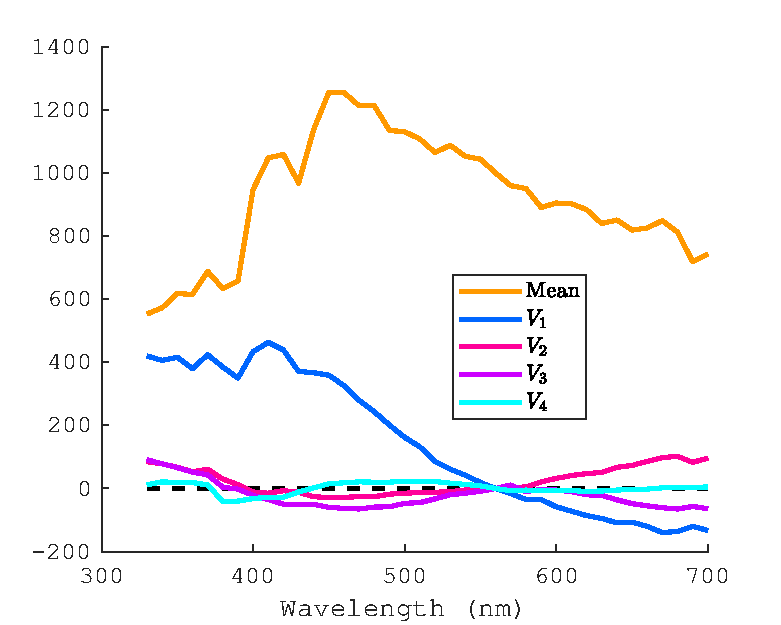
\includegraphics[max width=\textwidth]{figs/comp/LitRev/Judd.pdf}
 \caption{The mean and first four characteristic vectors of \citet{judd_spectral_1964}.}
 \label{fig:Judd}
\end{figure} 